%
% Article for Security RSA Cryptography
% Writed by: Stavros Papantonakis
%
%!TEX TS-program = xelatex
%!TEX encoding = UTF-8 Unicode
%
\documentclass[a4paper,12pt]{article}
	\usepackage{fontspec,xltxtra,xunicode}
	% Begin new paragraphs with an empty line rather than an indent
	\usepackage[greek]{babel}
	% justify paragraphs
	\usepackage[parfill]{parskip}
	\usepackage{xgreek}    
	%\usepackage{url}
	\usepackage{multirow}
	\usepackage{fancyvrb}
	\usepackage{colortbl}
	\usepackage{anyfontsize}
	\usepackage[usenames,dvipsname]{xcolor}
	\usepackage[colorlinks=true,linkcolor=black]{hyperref}
	\usepackage{pdfpages}
	\usepackage{ragged2e}
	\usepackage{babel}
	\usepackage{listings}
	\usepackage{amsmath}
	\usepackage{centernot}
	% Scaling based on Scale=MatchLowercase and Times New Roman
	% causes inconsistent output between OS X and FreeBSD
	% Therefore Scale is now set as an absolute number
	%\defaultfontfeatures{Scale=0.975,Mapping=tex-text}

	\newif\ifextrachapters
	
	
	%\defaultfontfeatures{Mapping=tex-text}	
	%\setromanfont[Mapping=tex-text]{Times New Roman}	
	\setmainfont[Mapping=tex-text]{GFS Didot}
	\usepackage{multicol}
	\usepackage{graphicx}
	\setcounter{secnumdepth}{4}
	\setcounter{tocdepth}{4}
	\usepackage{fancyhdr}
	\pagestyle{fancy}
	\fancyhf{}

	\fancyhead[LE,RO]{\bfseries\thepage}
	\fancyhead[LO]{\bfseries\rightmark}
	\fancyhead[RE]{\bfseries\leftmark}

	\renewcommand{\headrulewidth}{0.5pt}
	\addtolength{\headheight}{2pt}
	\renewcommand{\footrulewidth}{0pt}
	\addtolength{\headheight}{0.5pt}
	
	\fancypagestyle{plain}{%
	\fancyhead{}
	\renewcommand{\headrulewidth}{0pt}}
	
	%
	% User defined environments and commands
	%
	
	\newenvironment{inthebox}{\line(1,0){390}\\} %
  		{\line(1,0){390}}
	\DefineVerbatimEnvironment{richverb}%
		{Verbatim}{commandchars=\|\[\], commentchar=\!}
	\newcommand{\boxline}{\line(1,0){390}\\}	
	
	\author{Παπαντωνακης Σταυρος}
	\title {Arduino Fire Car}
	\date{7/4/2020}
	%
	%	
\begin{document}
	%
	%\maketitle
	% Title page
	%
	
\includepdf[pages=-]{cover/cover}
	%
% Writed by: Stavros Papantonakis
%
%!TEX TS-program = xelatex
%!TEX encoding = UTF-8 Unicode
%
\begin{titlepage}
	\begin{center}
		\vspace{1cm}	
		\Huge	
		\textbf{ Remote Method Invocation  \\  (Java RMI),(Corba)}
		
		\vspace{0.5cm}
		\large
		Απομεμακρυσμένη Κλήση Διαδικασιών
		
		\vspace{1.5cm}
		\textbf{Παπαντωνάκης Σταύρος\\ CSE45227}
		\vfill
		
		Αναφορά Δευτερης εργαστηριακής άσκησης\\
		Εργαστήριο κατανεμημένων\\
		ΣΤ12
		
		\vspace{0.8cm}
		\begin{center}
			
\includegraphics[width=0.4\textwidth]{image/logo.jpg}		
		\end{center}
		\normalsize
		Τμήμα Μηχανικών Πληροφορικής και Υπολογιστών\\
		Πανεπιστήμιο Δυτικής Αττικής\\
		Αθηνά\\
		31/05/2020\\	
	\end{center}
\end{titlepage}
	%
	% Creative Commons 4.0 License
	%
	%
% CC 4.0 License translation test file
% Translated by: Manolis Kiagias
%
%!TEX TS-program = xelatex
%!TEX encoding = UTF-8 Unicode
%
\begin{center}
Copyright \copyright 2020 Παπαντώνακης Σταύρος\\
Το Παρόν Έργο παρέχεται υπό τους όρους της Άδειας:\\

\includegraphics[scale=0.2]{license/images/cc-logo}\\
\textbf{Αναφορά Δημιουργού-Μη Εμπορική Χρήση-Παρόμοια Διανομή 4.0 Διεθνής}\\
Το πλήρες κείμενο αυτής της άδειας είναι διαθέσιμο εδώ:\\
\url{http://creativecommons.org/licenses/by-nc-sa/4.0/}
\end{center}
\subsection*{Είστε ελεύθερος να:}
\noindent
\textbf{Διαμοιραστείτε} -- να αντιγράψετε και αναδιανείμετε το υλικό με οποιοδήπότε μέσο και μορφή.\\
\textbf{Προσαρμόσετε} -- να αναμείξετε, μετασχηματίσετε και να επεκτείνετε το υλικό.\\

Ο αδειοδότης δεν μπορεί να σας αφαιρέσει αυτές τις ελευθερίες όσο ακολουθείτε τους όρους της παρούσας άδειας.
\subsection*{Ύπο τους ακόλουθους όρους:}

\vspace{1em}
\noindent
\parbox{1.5cm}{
\includegraphics[scale=0.15]{license/images/cc_by_30}}
\parbox{10.5cm}{\textbf{Αναφορά Δημιουργού} -- Θα πρέπει να αναφέρετε \textbf{τον δημιουργό του έργου}, να παρέχετε σύνδεσμο προς αυτή την άδεια, και να \textbf{υποδείξετε τυχόν αλλαγές}. Μπορείτε να το κάνετε με οποιοδήποτε εύλογο μέσο, αλλά όχι με τρόπο που να υπονοεί ότι ο αδειοδότης επικροτεί εσάς ή τη χρήση του έργου από εσάς.}

\vspace{1em}
\noindent
\parbox{1.5cm}{
\includegraphics[scale=0.15]{license/images/cc_nc_30}}
\parbox{10.5cm}{\textbf{Μη Εμπορική Χρήση} --  Δεν μπορείτε να χρησιμοποιήσετε το υλικό για \textbf{εμπορικούς σκοπούς}.}

\vspace{1em}
\noindent
\parbox{1.5cm}{
\includegraphics[scale=0.15]{license/images/cc_sa_30}}
\parbox{10.5cm}{\textbf{Παρόμοια Διανομή}  -- Αν αναμείξετε, μετασχηματίσετε ή επεκτείνετε το υλικό, θα πρέπει να διανείμετε τις αλλαγές σας υπό την \textbf{ίδια άδεια} με το πρωτότυπο έργο.}

\vspace{1em}
\noindent
\parbox{1.5cm}{\ }
\parbox{10.5cm}{\textbf{Όχι επιπλέον περιορισμοί} -- Δεν μπορείτε να εφαρμόσετε νομικούς όρους ή \textbf{τεχνικά μέσα} που να περιορίζουν νομικά τους άλλους να πράξουν σύμφωνα με τις ελευθερίες αυτής της άδειας.}
\subsection*{Σημειώσεις:}
\noindent
Δεν χρειάζεται να ακολουθήσετε την άδεια για τμήματα του υλικού που θεωρούνται δημόσια γνώση (public domain) ή όπου η χρήση τους επιτρέπεται εξαιτίας μιας \textbf{εξαίρεσης ή περιορισμού}.\\

\noindent
Δεν δίνονται εγγυήσεις. Η άδεια ίσως να μη σας δίνει όλα τα δικαιώματα για την επιδιωκόμενη χρήση. Για παράδειγμα, επιπλέον δικαιώματα όπως \textbf{δημοσιότητα, ιδιωτικότητα, ή ηθικά δικαιώματα} μπορεί να επιβάλλουν περιορισμούς στη χρήση του υλικού.\\
\line(1,0){390}\\\\
\noindent
Το παρόν έργο στοιχειοθετήθηκε σε \XeLaTeX. Ο πηγαίος κώδικας του είναι διαθέσιμος στην παρακάτω τοποθεσία:
\begin{center}
\url{https://github.com/lardianos/Distributed}
\end{center}
\newpage	
	%
	%
	\tableofcontents		
	\newpage
	%% Writed by: Stavros Papantonakis
%
%!TEX TS-program = xelatex
%!TEX encoding = UTF-8 Unicode
%
\section*{Εισαγωγή}
%Aferesi kenou arxis paragrafou
\noindent
Ο κρυπτογραφικός αλγόριθµος Rivest-Shamir-Adelman (RSA) είναι ένα κρυπτοσύστηµα δηµοσίου κλειδιού. 
Είναι ένας ασύµµετρος κρυπτογραφικός αλγόριθµος όπου κάθε χρήστης διαθέτει δύο κλειδιά, ένα ιδιωτικό 
και ένα δηµόσιο. Χρησιµοποιεί στοιχεία από τη θεωρία των αριθµών και σε συνδυασµό µε τα ιδιαίτερα 
µεγάλου µεγέθους κλειδιάεπιτυγχάνει κρυπτογράφηση σε αριθµητική υπολοίπου που καθιστά αδύνατη 
την αποκρυπτογράφηση µε παραγοντοποίηση. Θεωρείται µέχρι σήµερα ένας ασφαλής κρυπτογραφικός αλγόριθµος.

	
	% Writed by: Stavros Papantonakis
%
%!TEX TS-program = xelatex
%!TEX encoding = UTF-8 Unicode
%
\setcounter{section}{0}
\section*{Γενικό Πλαίσιο}


\noindent
Σας ζητείται να φτιάξετε σε C έναν concurrent  server (διεργασία εξυπηρετητή) o οποίος ως έργο εξυπηρέτησης θα επιτελεί τους ακόλουθους υπολογισμούς (λαμβάνοντας ως εισόδους έναν πραγματικό αριθμό a και ένα διάνυσμα ακεραίων της μορφής \(Y (y1,y2,…,yn)\) μήκους n όπου το n θα το ορίζει ο χρήστης, και τις οποίες θα μπορούν να στέλνουν επαναληπτικά ένας ή περισσότεροι clients  / διεργασίες πελατών):

\begin{enumerate}
	\item Τη μέση τιμή του διανύσματος \(Y\) (επιστροφή: ένας πραγματικός αριθμός)
	\item Τη μέγιστη και την ελάχιστη τιμή του \(Y\) (επιστροφή: ένας πίνακας μήκους 2 ακεραίων)
	\item Το γινόμενο \(a*Y\) (επιστροφή: ένα διάνυσμα πραγματικών αριθμών μήκους \(n\))
\end{enumerate}

\noindent
Η επικοινωνία θα πρέπει να γίνεται μέσω TCP AF\_INET (Internet Domain) sockets. Η κάθε διεργασία socket-Client θα διαβάζει από το πληκτρολόγιο (επαναληπτικά, μέχρι να δηλώσει ο χρήστης ότι δεν επιθυμεί να συνεχίσει).
\begin{itemize}
	\item[(α)] την επιλογή του υπολογισμού που επιθυμεί ο χρήστης να γίνει (1,2,3)
	\item[(β)]  τα αντίστοιχα-απαραίτητα κατά περίπτωση δεδομένα \((n, Y, a)\), θα τα διοχετεύει στη διεργασία socket-Server και θα περιμένει να λάβει από αυτήν το αποτέλεσμα για να το τυπώσει στην οθόνη.
\end{itemize}


\noindent
Η διεργασία socket-Server θα δέχεται τα δεδομένα προς επεξεργασία από τις διεργασίες socket-Clients, και θα παράγει το αντίστοιχο αποτέλεσμα ΟΧΙ μέσω δικιάς του (τοπικής) συνάρτησης-υπολογισμού ΑΛΛΑ μέσω κατάλληλου Remote Procedure Call που θα υλοποιήσετε με τη βοήθεια του ONC RPC implementation. Θα πρέπει δηλαδή η διεργασία socket-Server (λειτουργώντας παράλληλα και ως RPC-Client) να καλεί (ανάλογα με την τιμή υπολογισμού που έστειλε ο χρήστης - 1,2,3) την αντίστοιχη ρουτίνα από έναν RPC-Server και να περιμένει το αντίστοιχο αποτέλεσμα από αυτόν (προκειμένου να το διοχετεύσει στη συνέχεια στον αντίστοιχο socket-Client).  

\noindent
Όσον αφορά το RPC-based μέρος της επικοινωνίας, θα πρέπει πρώτα να ορίσετε σωστά το απαιτούμενο ('.x') interface file (ορίζοντας μέσα σε αυτό τρεις ξεχωριστές συναρτήσεις-διαδικασίες (μία για κάθε έναν από τους τρεις υπολογισμούς που ζητούνται παραπάνω), στη συνέχεια να παράγετε αυτοματοποιημένα μέσω του rpcgen utility (και με βάση τα όσα διδαχθήκατε στο εργαστήριο) τόσο τα απαιτούμενα system modules (RPC-server-stub module και RPC-client-stub module) για την υλοποίηση των ζητούμενων RPCs, όσο και τα έτοιμα templates για τα δύο application modules της εφαρμογής σας (RPC-server-application module και RPC-client-application module), και ακολούθως: 

\begin{itemize}
	\item[(α)]να ολοκληρώσετε κατάλληλα τo RPC-server-application module (το οποίο θα επιτελεί τις βασικές εργασίες εξυπηρέτησης πάνω στα δεδομένα-παραμέτρους που θα στέλνει απομεμακρυσμένη ο RPC-Client/socket-Server).
	\item[(β)]να ολοκληρώσετε κατάλληλα επίσης το RPC-client-application module (μέσω του οποίου θα επιτελείται επί της ουσίας η κλήση της εκάστοτε απομεμακρυσμένης διαδικασίας) ενσωματώνοντας/συγχωνεύοντας το μεταξύ άλλων με τη βασική διεργασία socket-Server που περιγράφηκε παραπάνω.
\end{itemize}

\section{Απάντηση}

\noindent
\subsection{Client.x}
\noindent
Αρχικά δημιουργούμε στο αρχείο .x μια struct (data) για τα δεδομένα που θα στέλνουμε στης RPC Procedure 
και μια struct (res\_num) για τα δεδομένα που θα λαμβάνουμε πίσω. Στη struct data δηλώνουμε μια μεταβλητή τύπου
float a στη οποία θα τοποθετούμε την τιμή του a, ένα πινάκα int Y\(<>\) ο οποίος θα αρχικοποιείται 
και θα δεσμεύει μνήμη ανάλογα με την τιμή n που θα δίνει ο χρήστης, και μια τιμή int n στην οποία θα αποθηκεύετε 
το μέγεθος του πινάκα Y. Για την struct res\_num θα χρειαστούμε μια float a\_res στην οποία θα αποθηκεύεται το
αποτέλεσμα του μέσου ορού. Έναν int maxmin[2] στον οποίο θα αποθηκεύεται το max και το min, και έναν float Υ\(<>\)
στον οποίο θα αποθηκεύεται το διάνυσμα αφότου έχει πολλαπλασιαστή με το a. Τέλος θα χρειαστούμε 3 procedures
ένα για κάθε λειτουργιά, τα οποία επιστρέφουν ένα struct res\_num για με τα αντίστοιχα αποτελέσματα και ως είσοδο
μια struct data με τα δεδομένα προς υπολογισμό. 

\begin{center}
			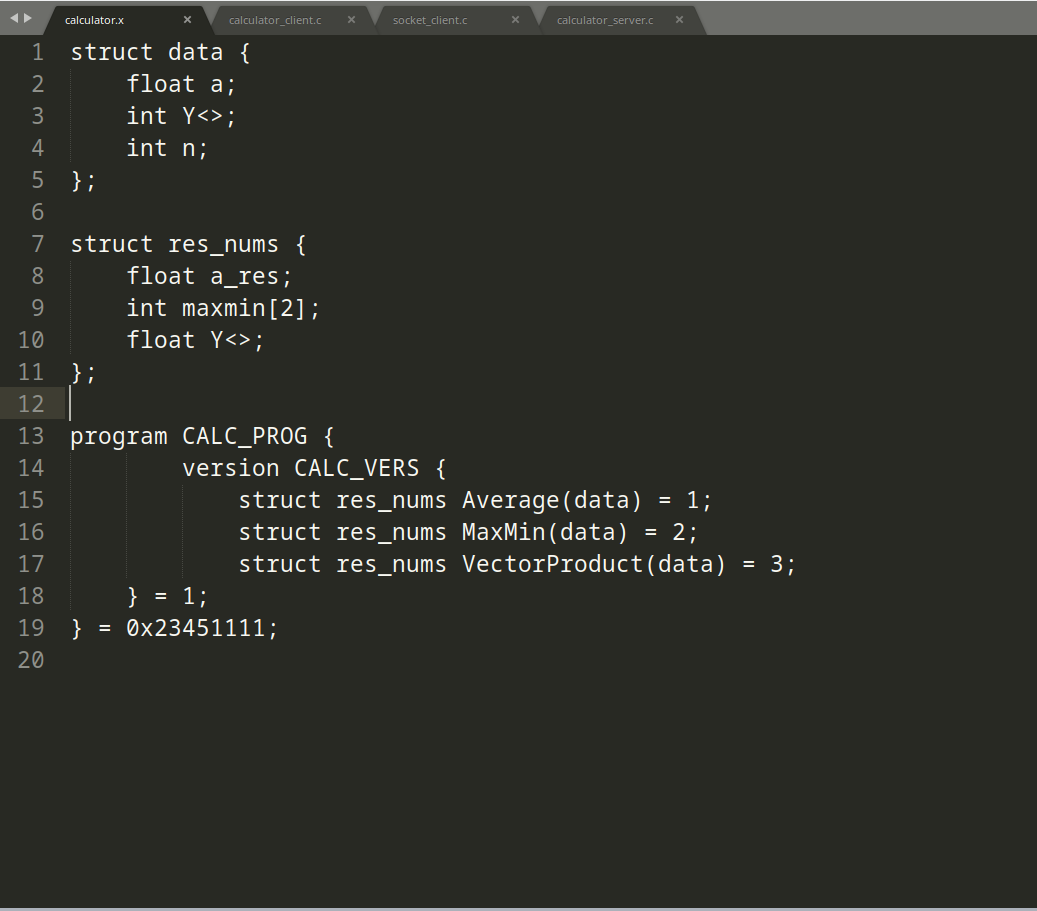
\includegraphics[width=1\textwidth]{image/calc-x.png}		
\end{center}

\noindent
Αμέσως μετά τρέχουμε την rpcgen και μας παράγει όλα τα απαραίτητα αρχεία. 

\subsection{Calculator (RPC Server)}
\noindent
Ανοίγουμε το αρχείο του RPC server
και γράφουμε τον κώδικα που που απαιτείτε για την υλοποίηση της average, maxmin και vectorproduct. Αρχικά για 
την  avergae δηλώνουμε μεταβλητές και θέτουμε τιμές σε αυτές. τρέχουμε ένα for loop και αθροίζουμε της 
τιμές του Y και τέλος υπολογίζουμε των μεσώ όρο, τον αναθέτουμε στον result.a\_res και επιστρέφουμε το result.

\begin{center}
			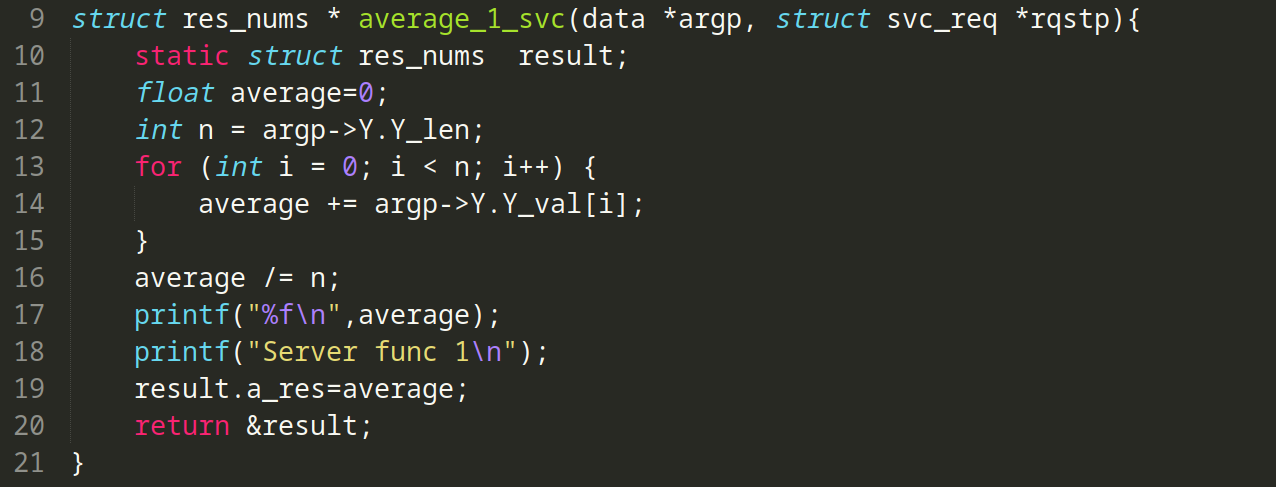
\includegraphics[width=1\textwidth]{image/average.png}		
\end{center}
\noindent
Για την maxmin αναθέτουμε τιμές σε μεταβλητές, τρέχουμε ενα for loop και υπολογίζουμε το max και το min του πινάκα
Y, το max το αναθέτουμε στο result.maxmin[0] και το min στο result.maxmin[1], τελειώνοντας επιστρέφουμε το result.

\begin{center}
			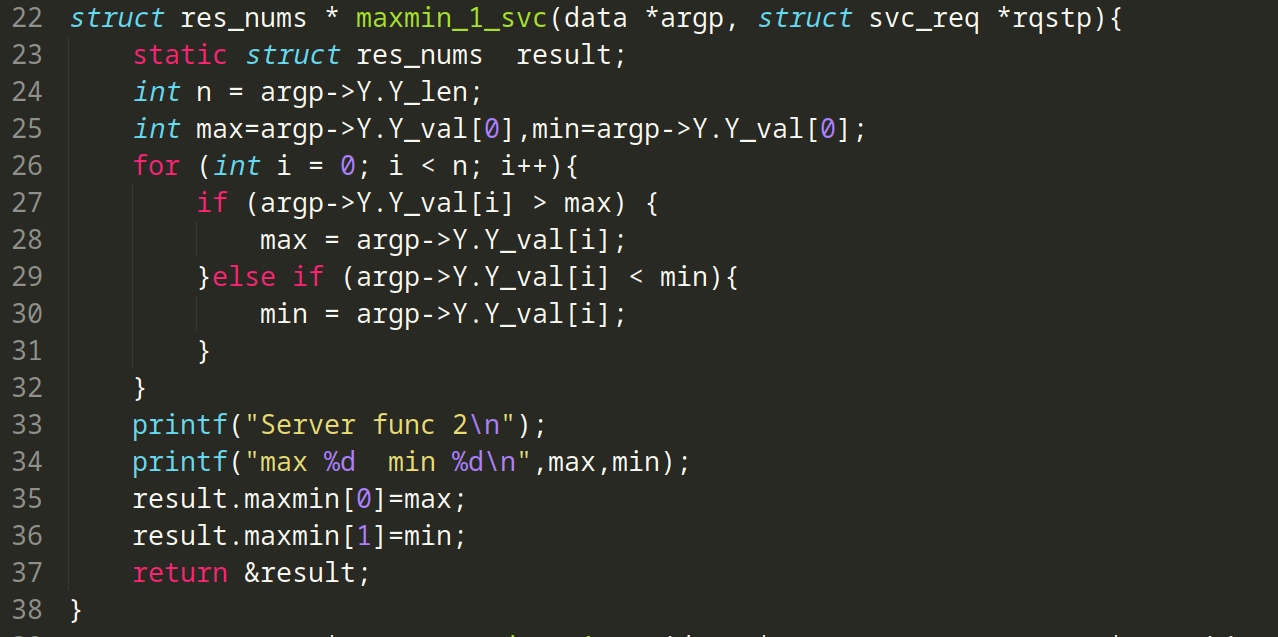
\includegraphics[width=1\textwidth]{image/maxmin.png}		
\end{center}
\noindent
Τέλος για την vectorproduct ακολουθάμε την ίδια διαδικασία  δηλώνοντας μεταβλητές και αναθέτοντας τιμές.
Σε αυτήν τη περίπτωση για την αποθήκευση τον αποτελεσμάτων χρησιμοποιήσουμε τον πινάκα Y της struct για αυτόν τον
λόγο δεσμεύουμε n θέσης στην μνήμη, υπολογίζουμε της τιμές και επιστρέφουμε το result.

\begin{center}
			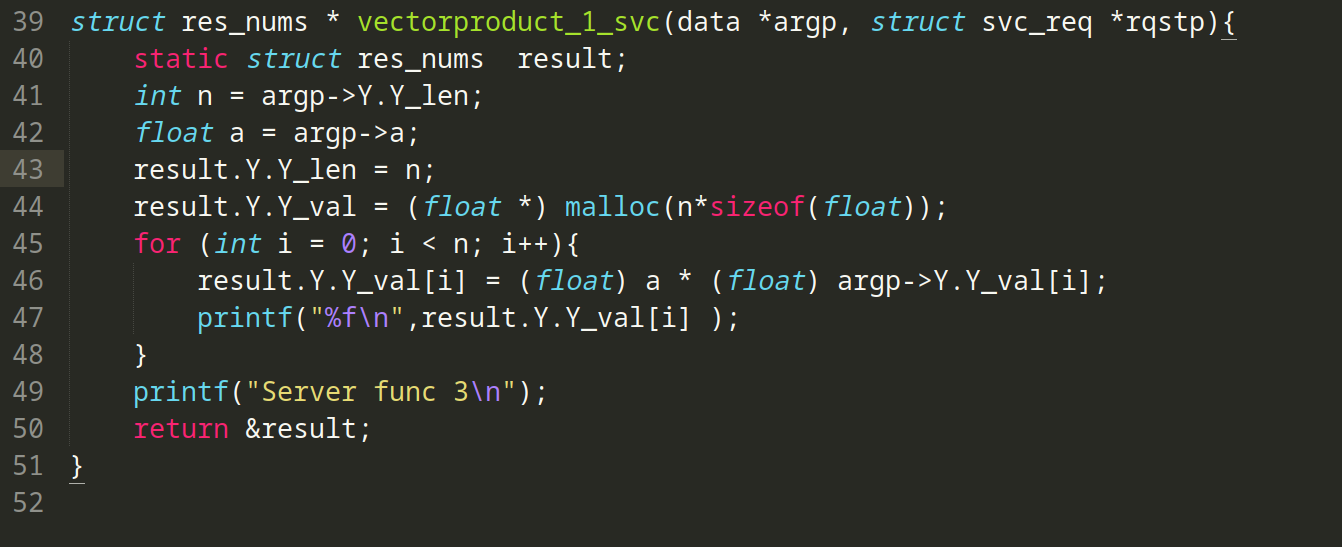
\includegraphics[width=1\textwidth]{image/vector.png}		
\end{center}

\subsection{Calculator (RPC Client/Socket Server)}
\noindent
Σε αυτό και στο επόμενο section δεν έχω χρησιμοποίηση screenshots λόγο της μεγάλης έκτασης του κώδικα,
θα προσπαθήσω να το εξηγήσω πως λειτουργεί μόνο με λογία.

\noindent
Αρχικά ο έτυμος κώδικας που παράχθηκε απο το rpcgen για των RPC Client, οταν καλειτε η calc\_prog\_1 καλουνται 
και η τρεις RPC procedures. επομένως προσθέτουμε μια λογική τριών if, οπού η κάθε μια ελέγχει μια μεταβλητή select
για το αν είναι 1,2 η 3 το όπιο select το προσθέτουμε στα inputs της calc\_prog\_1 για να το λαμβάνουμε όταν την
καλούμε. Σε κάθε μια από της if κάνουμε της απαραίτητες δεσμεύσεις χορού στην μνήμη και ανάθεσης τιμών στης
μεταβλητές της struct data. 

\noindent
Στην συνεχεία δημιουργούμε 3 struct που θα μας βοηθήσουν να αποθηκεύουμε δεδομένα και να τα περνάμε ανάμεσα στης
συναρτήσεις μας.
\begin{center}
	\begin{lstlisting}	
struct data_save{
	float a;
	int * Y;
	int n;	
};

struct addres_data{
	struct sockaddr_in addr;
	int len;
	int *newsockfd;
	char * s_host;	
};

typedef struct {
	float a_res;
	int maxmin[2];	
	float *Y;
	int Y_len;
}res_nums_cl;
	\end{lstlisting}	
\end{center}

\noindent
Παρατηρούμε ότι ο έτυμος κώδικας που έχει παραχθεί, ακολουθεί ένα μοτίβο. Αν στο 
αρχείο .x είχαμε δηλώσει περισσότερα programs με procedures θα μας είχε εμφάνιση περισσότερες functions της μορφής
calc\_prog\_1, calc\_prog\_2, calc\_prog\_3 κλπ. Παρόμοιο μοτίβο βλέπουμε και στης struct μεταβλητές εισόδου και
επιστροφής που δηλώνει πχ result\_1, result\_2, result\_3, average\_1\_arg, maxmin\_1\_arg, vectorproduct\_1\_arg. 
Κοιτάζοντας στο αρχείο .h παρατηρούμε ότι οι πινάκες της μορφής Y\(<>\) δηλώνονται ως μια struct που περιεχέι 
έναν pointer αντιστοίχου τύπου καθώς και μια μεταβλητή για την αποθηκεύσει του μήκους. 

\noindent
Για την αρχικοποίηση των δεδομένων μέσα στην calc\_prog\_1 προσθέτουμε στην είσοδο της μερικά πράγματα ακόμα 
όπως την float n\_num, την int n\_num και την int * y\_table. της οποίες θα της χρησιμοποιήσουμε για να περάσουμε 
τα δεδομένα μας σε αυτήν. Επίσης αλλάζουμε τον τύπο επιστροφής από void σε res\_nums\_c1 (σχόλιο: εδώ θα απορείτε
βεβαία γιατί φτιάξαμε της struct data\_save και res\_num\_cl ενώ θα μπορούσαμε να χρησιμοποιήσουμε της ήδη
υπάρχουσες του αρχείου .h καθώς είναι όμοιες, η απάντηση είναι ότι κάλλιστα θα μπορούσαμε να το κάνουμε άλλα
υπάρχει ένα βασικό πρόβλημα, δεν το σκεφτήκαμε όταν γράφαμε των κώδικα... ).

\noindent
Τέλος αφότου καλέσουμε την κάθε μια από αυτές της συναρτήσεις και μας επιστρέψουν τα αποτελέσματα, τα αναθέτουμε
σε μια μεταβλητή struct res\_num\_cl ret1 και τα επιστρέφουμε μεσώ του return.

\noindent
Στην συνεχεία φτιάχνουμε μια νέα συνάρτηση void * reciveMessage(void * cli\_data) όπου θα υλοποιεί την βασική
λειτουργιά του προγράμματος οπού την εκτελούν threads μεσώ της pthread\_create() και παίρνει ως είσοδο έναν void
pointer, εμείς στον void pointer αναθέτουμε έναν struct pointer της δομής addres\_data οπού περιεχέι κάποια
βασικά δεδομένα για την επικοινωνία με των σωστό client καθώς και το socket, οπός την διεύθυνση του client 
τον file descriptore του socket και την διεύθυνση του RPC server. αρχικά δηλώνουμε κάποιες μεταβλητές, flags κλπ.
Δεν έχει νόημα να της αναλύσουμε όλες μια μια, η περισσότερες εξάλλου φαίνεται τη κάνουν από το όνομα τους. Αυτές που έχει νόημα να αναφέρουμε είναι η struct data\_save data; στην όπια αποθηκεύουμε τα δεδομένα αφού τα λάβουμε
από των socket client, την struct addres\_data * local\_address\_data = cli\_data; οπού αποθηκεύουμε τα δεδομένα
επικοινωνίας του client. των char buffer[BUF\_SIZE]; που θα χρησιμοποιήσουμε για να αποθηκεύσουμε τα δεδομένα
που μας στέλνει ο χρήστης και την res\_nums\_cl ret1; οπού θα πάρουμε τα δεδομένα άπω τα return της calc\_prog\_1.

\noindent
ο Βασικός κώδικας αυτής της συνάρτησης τρέχει σε έναν ατέρμον βρόχο οπού τερματίζει μόνο όταν πάρει από τον socket
client ως επιλογή λειτουργίας των χαρακτήρα '0'. Στην ουσία αυτό που κάνει είναι να εκτελεί τη recvfrom() οπού
περιμένει μέχρις ότου ο χρήστης του στήλη δεδομένα. μόλις τα λάβει ελέγχει αν ο πρώτος χαρακτήρας είναι ο 
χαρακτήρας '0', εάν είναι εκτελεί return(void *)"END"; και τερματίζει την συνάρτηση. Σε διαφορετική περίπτωση 
έχουμε φτιάξει έναν κώδικα από μερικά for loops τα οποία κάνουν extract τα δεδομένα από τον buffer, τα 
μετατρέπουν από string σε διαχειρίσιμα δεδομένα(int, float κλπ.) έτσι ώστε να μπορούμε να τα αποστείλουμε στην 
calc\_prog\_1. αμέσως μετά έχουμε 3 if οπού επιλεγούν ανάλογα με το select τη δεδομένα θα στείλουν στην calc\_prog\_1. Αφότου εκτελεστή η calc\_prog\_1 επιστρέφει την ανάλογη struct με τα αποτελέσματα στο ret1. Τέλος 
μετατρέπουμε τα αποτελέσματα ξανά σε string με την sprintf() και τα τοποθετούμε σε έναν buffer με την strcat()
και τα αποστέλλουμε στον socket client με την sendto(). Τέλος ξαναγυρίζουμε στην αρχή και περιμένουμε να μας
ξαναστείλει ο χρήστης δεδομένα.

\noindent
Στην main ο έτυμος κώδικας χρησιμοποιεί argv είσοδο για την διεύθυνση του RPC Server. Για να φταίξουμε την 
επικοινωνία με τα Socket δηλώνουμε 2 ακεραίους οπού θα αποθηκευτούν τα file descriptores που θα δημιουργηθούν.
Εκτελούμε την sockfd=socket(AF\_INET,SOCK\_STREAM,0); και δημιουργούμε ένα socket, άμεσος μετά τρέχουμε την
setsockopt(sockfd, SOL\_SOCKET, SO\_REUSEADDR,\&yes, sizeof(int)) για να σετάρουμε το socket. Αναθέτουμε τιμές 
στο struct του socket.

\begin{center}
	\begin{lstlisting}	
memset(&addr,0,sizeof(addr));
addr.sin_family =AF_INET;
addr.sin_addr.s_addr=INADDR_ANY;
addr.sin_port=PORT;
	\end{lstlisting}	
\end{center}

\noindent
Στην συνεχια κανουμε bind() και listen() και περιμενουμε για connect με την 
newsockfd=accept(sockfd, (struct sockaddr*) \&cl\_addr, (socklen\_t*) \&len); μόλις γίνει το accept αποθηκεύουμε
την διεύθυνση του του client και το fd του socket του στην δομή struct addres\_data cl\_data και δημιουργούμε ένα
thread με την pthread\_create το οποίο καλή την reciveMessage και της περνάει την δομή cl\_data και
ξαναπαίρνουμε για connect από άλλο client. 


\subsection{Socket Client}
\noindent
Στον client έχουμε δημιουργήσει μια συνάρτηση keyboard\_read() που την χρησιμοποιούμε για να διαβάσουμε χαρακτήρες
από το πληκτρολόγιο, μια συνάρτηση num\_control για να ελέγχουμε αν οι χαρακτήρες που έδωσε ο χρήστης είναι
αποδεκτοί, μια συνάρτηση receiveMessage που αποτυπώνει ότι στέλνει RPC Clinet/Socket Server. Και τέλος μια
συνάρτηση μενού η οποία παρουσιάζει το μενού με της επιλογές του χρήστη, διαβάζει τα δεδομένα από το πληκτρολόγιο
και τα αποθηκεύει στην δομή data\_save και το κάνουμε return. 

\begin{center}
	\begin{lstlisting}	
typedef struct{
    char select;
    char * a_value;
    char * Y_value;
    char * n_value; 
    int n_length;
    int Y_length; 
    int a_length;
}data_save;
	\end{lstlisting}	
\end{center}

\noindent
Στην main τώρα κάνουμε την αντιστοιχεί διαδικασία με των Socket Server, απλά αντί για accept() κάνουμε connect()
και ανάλογα τι επιλογή διαμορφώνουμε τα δεδομένα σε έναν πινάκα χαρακτήρων τις μορφής char buf[]=[select;n;Y.value[0],Y.value[1],Y.value[2]....Y.value[n];a] των οποίο προωθούμε στην sendto() και καλούμε
την recive περιμένοντας τα αποτελέσματα. 

\noindent


\noindent


\noindent

\noindent

\noindent

\noindent


\end{document}